%===============================================================================
% LaTeX sjabloon voor de bachelorproef toegepaste informatica aan HOGENT
% Meer info op https://github.com/HoGentTIN/latex-hogent-report
%===============================================================================

\documentclass[dutch,dit,thesis]{hogentreport}

% TODO:
% - If necessary, replace the option `dit`' with your own department!
%   Valid entries are dbo, dbt, dgz, dit, dlo, dog, dsa, soa
% - If you write your thesis in English (remark: only possible after getting
%   explicit approval!), remove the option "dutch," or replace with "english".

\usepackage{lipsum} % For blind text, can be removed after adding actual content

%% Pictures to include in the text can be put in the graphics/ folder
\graphicspath{{graphics/}}

%%---------- Document metadata -------------------------------------------------
% TODO: Replace this with your own information
\author{Laurent Duquesnoy}
\supervisor{Dhr. J. Claes}
\cosupervisor{Mr. S. Dewolf}
\title%
    {Deltalex advocaten - Optimalisatie van de administratieve workflow in juridische kantoren: automatisering van repetitieve taken}
\academicyear{\advance\year by -1 \the\year--\advance\year by 1 \the\year}
\examperiod{1}
\degreesought{\IfLanguageName{dutch}{Professionele bachelor in de toegepaste informatica}{Bachelor of applied computer science}}
\partialthesis{false} %% To display 'in partial fulfilment'
%\institution{Internshipcompany BVBA.}

%% Add global exceptions to the hyphenation here
\hyphenation{back-slash}

%% The bibliography (style and settings are  found in hogentthesis.cls)
\addbibresource{bachproef.bib}            %% Bibliography file
\addbibresource{../voorstel/voorstel.bib} %% Bibliography research proposal
\defbibheading{bibempty}{}

%% Prevent empty pages for right-handed chapter starts in twoside mode
\renewcommand{\cleardoublepage}{\clearpage}

\renewcommand{\arraystretch}{1.2}

%% Content starts here.
\begin{document}

%---------- Front matter -------------------------------------------------------

\frontmatter

\hypersetup{pageanchor=false} %% Disable page numbering references
%% Render a Dutch outer title page if the main language is English
\IfLanguageName{english}{%
    %% If necessary, information can be changed here
    \degreesought{Professionele Bachelor toegepaste informatica}%
    \begin{otherlanguage}{dutch}%
       \maketitle%
    \end{otherlanguage}%
}{}

%% Generates title page content
\maketitle
\hypersetup{pageanchor=true}

%%=============================================================================
%% Voorwoord
%%=============================================================================

\chapter*{\IfLanguageName{dutch}{Woord vooraf}{Preface}}%
\label{ch:voorwoord}

%% TODO:
%% Het voorwoord is het enige deel van de bachelorproef waar je vanuit je
%% eigen standpunt (``ik-vorm'') mag schrijven. Je kan hier bv. motiveren
%% waarom jij het onderwerp wil bespreken.
%% Vergeet ook niet te bedanken wie je geholpen/gesteund/... heeft

Beste lezer, als u dit leest hebt u een kopie bemachtigd van mijn bachelorthesis. 
Ik zou eerst en vooral mijn promotor, de heer Jan Claes van HoGent en mijn co-promotor, Stijn Dewolf van Deltalex van harte willen bedanken voor de goede ondersteuning en behulpzaamheid tijdens dit project. 


Dit is een thesis geschreven door een student die een passie heeft in het gebied van Informatietechnologie en er al heel zijn leven mee bezig is. 
Deze passie heeft mij toegelaten om te denken als een problem solver en problemen rond mij te zoeken, vast te stellen en vervolgens te proberen er een oplossing voor te bedenken. 
Het probleem dat ik in deze thesis zal bestuderen is het probleem van repetitie op de werkvloer, meer specifiek in een advocatenkantoor genaamd Deltalex. 
Ik merkte op dat er daar heel veel taken gebeuren die gigantisch repetitief zijn in aard. 
Als programmeur denk ik altijd na om veel meer tijd te besteden om een bepaalde taak te automatiseren dan deze manueel af te handelen, logischerwijs dacht ik dan ook om dit probleem eens onder de loep te nemen. 
Mogelijke oplossingen die mij te binnen schoten waren plugins in document editors (b.v. Word), custom document macro's e.d. 

Na wat feedback van mijn promotor ben ik op het idee gekomen om een digitale assistent te bouwen om de advocaten in allerlei administratieve taken bij te staan. 

Nu is het probleem dat er bij advocaten heel veel gewerkt wordt met confidentiële data. 
Het is dus imperatief dat de data van cliënten nooit de veilige omgeving van Deltalex verlaat. 
Deze proef zal dus blijven bij hypothetische research over het bouwen van de ideale digitale assistent. 
De bedoeling van deze thesis is dus om u, de lezer, zo goed mogelijk te informeren en weg te wijzen in het bouwen en onderhouden van een digitale assistent. 
Ik hoop om u dan ook zo veel mogelijk te leren en de weg te wijzen tijdens dit avontuur van optimalisatie van taken en de verkenning van Artificiële intelligentie. 

%%=============================================================================
%% Samenvatting
%%=============================================================================

% TODO: De "abstract" of samenvatting is een kernachtige (~ 1 blz. voor een
% thesis) synthese van het document.
%
% Een goede abstract biedt een kernachtig antwoord op volgende vragen:
%
% 1. Waarover gaat de bachelorproef?
% 2. Waarom heb je er over geschreven?
% 3. Hoe heb je het onderzoek uitgevoerd?
% 4. Wat waren de resultaten? Wat blijkt uit je onderzoek?
% 5. Wat betekenen je resultaten? Wat is de relevantie voor het werkveld?
%
% Daarom bestaat een abstract uit volgende componenten:
%
% - inleiding + kaderen thema
% - probleemstelling
% - (centrale) onderzoeksvraag
% - onderzoeksdoelstelling
% - methodologie
% - resultaten (beperk tot de belangrijkste, relevant voor de onderzoeksvraag)
% - conclusies, aanbevelingen, beperkingen
%
% LET OP! Een samenvatting is GEEN voorwoord!

%%---------- Nederlandse samenvatting -----------------------------------------
%
% TODO: Als je je bachelorproef in het Engels schrijft, moet je eerst een
% Nederlandse samenvatting invoegen. Haal daarvoor onderstaande code uit
% commentaar.
% Wie zijn bachelorproef in het Nederlands schrijft, kan dit negeren, de inhoud
% wordt niet in het document ingevoegd.

\IfLanguageName{english}{%
\selectlanguage{dutch}
\chapter*{Samenvatting}
\selectlanguage{english}
}{}

%%---------- Samenvatting -----------------------------------------------------
% De samenvatting in de hoofdtaal van het document

\chapter*{\IfLanguageName{dutch}{Samenvatting}{Abstract}}

In kantoren met een grote administratieve workload, zoals een advocatenkantoor, bestaat er een heel grote kans dat er een heel groot aantal aan documenten 
in het archief en verschillende databanken resideert. 

Het is niet altijd makkelijk voor advocaten en medewerkers om zich aan te passen aan het snel evoluerende klimaat van informatietechnologie omdat zij zich vooral 
focussen op het (ook snel evoluerende) rechtssysteem.

Zodoende stagneert (of evolueert) de kwaliteit van de ondersteuning, maar de productiviteit daarentegen kan verlagen. 
Daarom kan het handig zijn voor dergelijke kantoren om te investeren in een systeem dat dienst kan doen als een digitale assistent. 

Deze bachelorproef gaat over de implementatiestappen van dergelijk systeem. Hij is verdeeld in in verschillende stappen. 

Deze stappen zullen de rode draad vormen in deze proef en gaan over een analyse van het kantoor en mogelijke bottlenecks, het vergaren van trainingdata, het bouwen van een model en interface
voor advocaten om te werken met een tool die uiteindelijk hun productiviteit zal verhogen. Hiervoor wordt een Large Language Model geïntegreerd om natuurlijke taal te vertalen naar 
systeemrequests. 

Ook zal er analyse gedaan worden naar welke technologieën er voor handen zijn en welke er het best passen bij de toepassingen. Bijvoorbeeld zal er onderzocht worden welk type database
het snelst kan omgaan met de data die gebruikt wordt, welke plugins er kunnen gebruikt worden om te integreren in bestaande programma's, welke interfaces het makkelijkst zijn enz. 

Ook wordt via de eerste analyse bekeken welke toepassingen haalbaar zijn in het tijdskader van 12 weken. 

Achteraf volgt een korte analyse, die stukken van het Business Acceptance Model gebruikt om te schetsen wat de impact is.



%---------- Inhoud, lijst figuren, ... -----------------------------------------

\tableofcontents

% In a list of figures, the complete caption will be included. To prevent this,
% ALWAYS add a short description in the caption!
%
%  \caption[short description]{elaborate description}
%
% If you do, only the short description will be used in the list of figures

\listoffigures

% If you included tables and/or source code listings, uncomment the appropriate
% lines.
%\listoftables
%\listoflistings

% Als je een lijst van afkortingen of termen wil toevoegen, dan hoort die
% hier thuis. Gebruik bijvoorbeeld de ``glossaries'' package.
% https://www.overleaf.com/learn/latex/Glossaries

%---------- Kern ---------------------------------------------------------------

\mainmatter{}

% De eerste hoofdstukken van een bachelorproef zijn meestal een inleiding op
% het onderwerp, literatuurstudie en verantwoording methodologie.
% Aarzel niet om een meer beschrijvende titel aan deze hoofdstukken te geven of
% om bijvoorbeeld de inleiding en/of stand van zaken over meerdere hoofdstukken
% te verspreiden!

%%=============================================================================
%% Inleiding
%%=============================================================================

\chapter{\IfLanguageName{dutch}{Inleiding}{Introduction}}%
Deze bachelorproef handelt over het verbeteren van de efficiëntie van administratieve taken bij advocatenkantoren.
De natuur van de taken die deze beoogt te verbeteren zijn veelal repetitief in aard.
Dit onderzoek ontspringt zich in de observatie dat bepaalde taken die uitgevoerd worden frustrerend en traag zijn.
Een digitale assistent kan de tijd die deze taken innemen minimaliseren en het mogelijk maken deze te herinvesteren in taken die meer uitdagend en variërend zijn.

\section{\IfLanguageName{dutch}{Probleemstelling}{Problem Statement}}%
\label{sec:probleemstelling}

Als we kijken bij de administratieve backend in Deltalex advocaten en observeren hoe bepaalde taken gebeuren, valt op dat veel taken die uitgevoerd worden repetitief en tijdrovend zijn.
Deze taken kunnen impact hebben op de productiviteit van medewerkers, de herhalende aard van de taken vergroot
ook de kans op fouten die makkelijk overzien worden maar een grote impact kunnen hebben op het kantoor.
Denk maar aan foute looncalculaties, miscommunicatie, spelfouten, \dots
Natuurlijk is het niet eenvoudig om een automatisatie toe te passen op een heel specifiek punt, deze bachelorproef zal deels dienen als een Proof Of Concept om de haalbaarheid van
dergelijke tools in een geavanceerde kantooromgeving te illustreren.

\section{\IfLanguageName{dutch}{Onderzoeksvraag}{Research question}}%
\label{sec:onderzoeksvraag}

Uit de bovenstaande passage ontspringt de vraag:
"Bestaat er een mogelijkheid om repetitieve taken te automatiseren?
Kan een dergelijke toepassing de productiviteit van een advocaat positief beïnvloeden?
Hoe haalbaar is een dergelijke toepassing?
Kan deze dienen als vervanging van de manuele uitvoer van zulke taken?".

\section{\IfLanguageName{dutch}{Onderzoeksdoelstelling}{Research objective}}%
\label{sec:onderzoeksdoelstelling}
Wat is het beoogde resultaat van je bachelorproef?
Wat zijn de criteria voor succes? Beschrijf die zo concreet mogelijk. Gaat het bv. om een proof-of-concept, een prototype, een verslag met aanbevelingen, een vergelijkende studie, enz.

Het beoogde resultaat van deze bachelorproef kan opgedeeld worden in zes delen:
\begin{itemize}
	\item Het versnellen en verbeteren van de workflow van advocaten die werkzaam zijn bij Deltalex
    \item Het analyseren van de data (dossiers, communicatie, documenten) die gebruikt kan worden voor optimalisatie
    \item Naast een digitale assistent, een potentiële snelle, geoptimaliseerde zoekmachine voor hun documentendatabase
    \item De haalbaarheid van deze features in kaart brengen
    \item Aantonen via onderzoek of een dergelijke implementatie concrete voordelen heeft op de manuele executie van taken
\end{itemize}


\section{\IfLanguageName{dutch}{Opzet van deze bachelorproef}{Structure of this bachelor thesis}}%
\label{sec:opzet-bachelorproef}

% Het is gebruikelijk aan het einde van de inleiding een overzicht te
% geven van de opbouw van de rest van de tekst. Deze sectie bevat al een aanzet
% die je kan aanvullen/aanpassen in functie van je eigen tekst.

De rest van deze bachelorproef is als volgt opgebouwd:

In Hoofdstuk~\ref{ch:stand-van-zaken} wordt een overzicht gegeven van de stand van zaken binnen het onderzoeksdomein, op basis van een literatuurstudie.

In Hoofdstuk~\ref{ch:methodologie} wordt de methodologie toegelicht en worden de gebruikte onderzoekstechnieken besproken om een antwoord te kunnen formuleren op de onderzoeksvragen.

% TODO: Vul hier aan voor je eigen hoofstukken, één of twee zinnen per hoofdstuk

In Hoofdstuk~\ref{ch:conclusie}, tenslotte, wordt de conclusie gegeven en een antwoord geformuleerd op de onderzoeksvragen. Daarbij wordt ook een aanzet gegeven voor toekomstig onderzoek binnen dit domein.

\chapter{\IfLanguageName{dutch}{Stand van zaken}{State of the art}}%
\label{ch:stand-van-zaken}

% Tip: Begin elk hoofdstuk met een paragraaf inleiding die beschrijft hoe
% dit hoofdstuk past binnen het geheel van de bachelorproef. Geef in het
% bijzonder aan wat de link is met het vorige en volgende hoofdstuk.

% Pas na deze inleidende paragraaf komt de eerste sectiehoofding.

Dit hoofdstuk bevat je literatuurstudie. De inhoud gaat verder op de inleiding, maar zal het onderwerp van de bachelorproef *diepgaand* uitspitten.
De bedoeling is dat de lezer na lezing van dit hoofdstuk helemaal op de hoogte is van de huidige stand van zaken (state-of-the-art) in het onderzoeksdomein.
Iemand die niet vertrouwd is met het onderwerp, weet nu voldoende om de rest van het verhaal te kunnen volgen, zonder dat die er nog andere informatie moet over opzoeken \autocite{Pollefliet2011}.

Je verwijst bij elke bewering die je doet, vakterm die je introduceert, enz.\ naar je bronnen. In \LaTeX{} kan dat met het commando \texttt{$\backslash${textcite\{\}}} of \texttt{$\backslash${autocite\{\}}}. Als argument van het commando geef je de ``sleutel'' van een ``record'' in een bibliografische databank in het Bib\LaTeX{}-formaat (een tekstbestand). Als je expliciet naar de auteur verwijst in de zin (narratieve referentie), gebruik je \texttt{$\backslash${}textcite\{\}}. Soms is de auteursnaam niet expliciet een onderdeel van de zin, dan gebruik je \texttt{$\backslash${}autocite\{\}} (referentie tussen haakjes). Dit gebruik je bv.~bij een citaat, of om in het bijschrift van een overgenomen afbeelding, broncode, tabel, enz. te verwijzen naar de bron. In de volgende paragraaf een voorbeeld van elk.

\textcite{Knuth1998} schreef een van de standaardwerken over sorteer- en zoekalgoritmen. Experten zijn het erover eens dat cloud computing een interessante opportuniteit vormen, zowel voor gebruikers als voor dienstverleners op vlak van informatietechnologie~\autocite{Creeger2009}.

Let er ook op: het \texttt{cite}-commando voor de punt, dus binnen de zin. Je verwijst meteen naar een bron in de eerste zin die erop gebaseerd is, dus niet pas op het einde van een paragraaf.


\section{Inefficiënt documentmanagement en repetitie}
\label{sec:documentmanagement}

\subsection{Repetitie}
In een advocatenkantoor is het vanzelfsprekend dat er heel veel administratie aan bod komt. Denk maar aan het opstellen van dagvaardingen,
ingebrekestellingen, e-mails, aangetekende brieven en andere communicatie.

Natuurlijk dringt zich dit op dat deze taken veel tijd in beslag kunnen nemen. Naast een administratief spectrum gaat het ook over verdediging van cliënten, pleiten en ander rechtbankwerk.

Moest er daar dan nog extra repetitief bureauwerk aan te pas komen, kan dit een obstakel vormen naar productiviteit toe. Hiervoor onderstaande citatie ter illustratie:
\begin{displayquote}
	\textit{"How much time is spent in repetitive tasks in the workplace? Today the typical office worker spends 10\% of their time on manual data entry into business applications,
		such as the ERP system, CRM or spreadsheets. In total, they spend over 50\% of work time creating or updating documents, eg. PDFs, spreadsheets or word documents \autocite{Workfellow}."}
\end{displayquote}

Natuurlijk is dit een generieke citatie die handelt over PDFs, spreadsheets en dergelijke, maar ze is zeker ook toepasbaar in een advocatenkantoor.

Het komt er op neer dat repetitie een killer is voor productiviteit omdat het juist zoveel tijd in beslag neemt,
volgende citatie handelt over het aantal copy pastes van een gemiddelde administratieve medewerker:

\begin{displayquote}
	\begin{itemize}
		\item \emph {A typical office worker spends 3 hours working on spreadsheets each week, for example in Microsoft Excel or Google Sheets.}
		\item \emph {A typical office worker spends almost 2 1/2 hours in business communications or email applications, such as Outlook.}
		\item \emph {A typical office worker spends over 1 1/2 hours each week searching and organizing files, for example in the shared file service such as Sharepoint or Google Drive.}
		\item \emph {A typical office worker spends 1 1/2 hours each week copy-pasting or manually entering data into business applications, such as the ERP or CRM.} \autocite{Workfellow}
	\end{itemize}
\end{displayquote}

\subsection{Het managen van grote hoeveelheden documenten}
Doorheen de jaren wordt er een heel groot archief aan documenten opgebouwd.
Het doorzoeken en onderhouden van dit archief kan voor velen een grote uitdaging vormen en ook heel veel tijd in beslag nemen,
dit kan de productiviteit van een kantoor in het gedrang brengen en heel tijdrovend zijn, zeker als het archief inefficiënt is opgebouwd.

Het opzoeken van documenten in een archief is een mooi voorbeeld om te vergelijken tussen menselijke en machinale zoekmethodes.
Het opzoeken van data in een archief kan parallel gesteld worden met een zoekmachine. Volgende citatie schetst oppervlakkig het verschil tussen
menselijke en digitale methodes.

\begin{displayquote}
	Search engines have been with us for several decades as an integral part of our digital life.
	We are casually searching over billions of web pages to retrieve and share information from various resources.
	While humans are very good at conversational context and background knowledge which helps them to deal with intrinsic ambiguity of words,
	it may not be true in case of search engines, especially when it comes to out-of-the-vocabulary searches \autocite{MediumSemanticSearch}
\end{displayquote}

Het artikel handelt verder over semantische zoekmethodes en schetst een voorbeeld met een voorbeeld-dataset en een proof-of-concept in Python.

Zoekmachines gebruikten echter niet altijd een semantische methodiek:

\begin{displayquote}
	At first, search engines were lexical: the search engine looked for literal matches of the query words,
	without understanding of the query’s meaning and only returning links that contained the exact query. \autocite{MediumSemanticSearch}
\end{displayquote}

Lexicaal zoeken is vrij simpel te implementeren en is een vrij primitief concept. Semantisch zoeken is daarentegen wat complexer te integreren:

\begin{displayquote}
	On the other hand, “Semantic Search” can simplify query building, because it is supported by automated natural language processing programs
	i.e. using Latent Semantic Indexing — a concept that search engines use to discover how a keyword and content work together to mean the same thing. \autocite{MediumSemanticSearch}
\end{displayquote}

Wat heeft dit nu te maken met documentmanagement? Een zoekmachine is een polyvalente tool die ingezet kan worden op verschillende datasets. Dit kan ook een volledig archief zijn van
documenten in een advocatenkantoor. Het implementeren van een semantisch zoekalgoritme kan een oplossing bieden op het eerste subprobleem: inefficiënt zoeken in dit archief.

\begin{displayquote}
	In brief, LSI(Latent Semantic Index) does not require an exact match to return useful results.
	Where a plain keyword search will fail if there is no exact match,
	LSI will often return relevant documents that don’t contain the keyword at all. \autocite{MediumSemanticSearch}
\end{displayquote}

\subsection{Obstakels in research van rechtszaken}
Bij een (oppervlakkige) verkennende audit bij advocatenkantoor Deltalex viel op dat er veel tijd wordt gespendeerd aan het opzoeken van dossiergerelateerde informatie. Denk hierbij maar aan
contactgegevens (ondernemingsnummer, adres, ...) van een cliënt, dossierdata, technische specificaties, enz.

Voor een advocaat kan dit een bijzonder lang en repetitief proces vormen indien manueel uitgevoerd. Gelukkig kunnen hier technieken zoals RAG (Retrieval-Augmented Generation) een grote hulp
bij bewijzen. RAG (Retrieval Augmented Generation) is een van de grootste use cases voor LLM's en is een framework dat de fundamentele trainingsdata van een Large Language Model
combineert met bestaande data in een database. Zodoende kan een model gegronde antwoorden geven, gebaseerd op betrouwbare en relevante informatie.

Een quote van Medium legt uit hoe RAG werkt in grote lijnen:

\begin{displayquote}
	A typical RAG process, as pictured below, has an LLM, a collection of enterprise documents, and supporting infrastructure to improve information retrieval and answer construction.
	The RAG pipeline looks at the database for concepts and data that seem similar to the question being asked, extracts the data from a vector database and reformulates the data into
	an answer that is tailored to the question asked. This makes RAG a powerful tool for companies looking to harness their existing data repositories for enhanced decision-making
	and information access. \autocite{MediumRAG}
	\begin{figure}[h]
		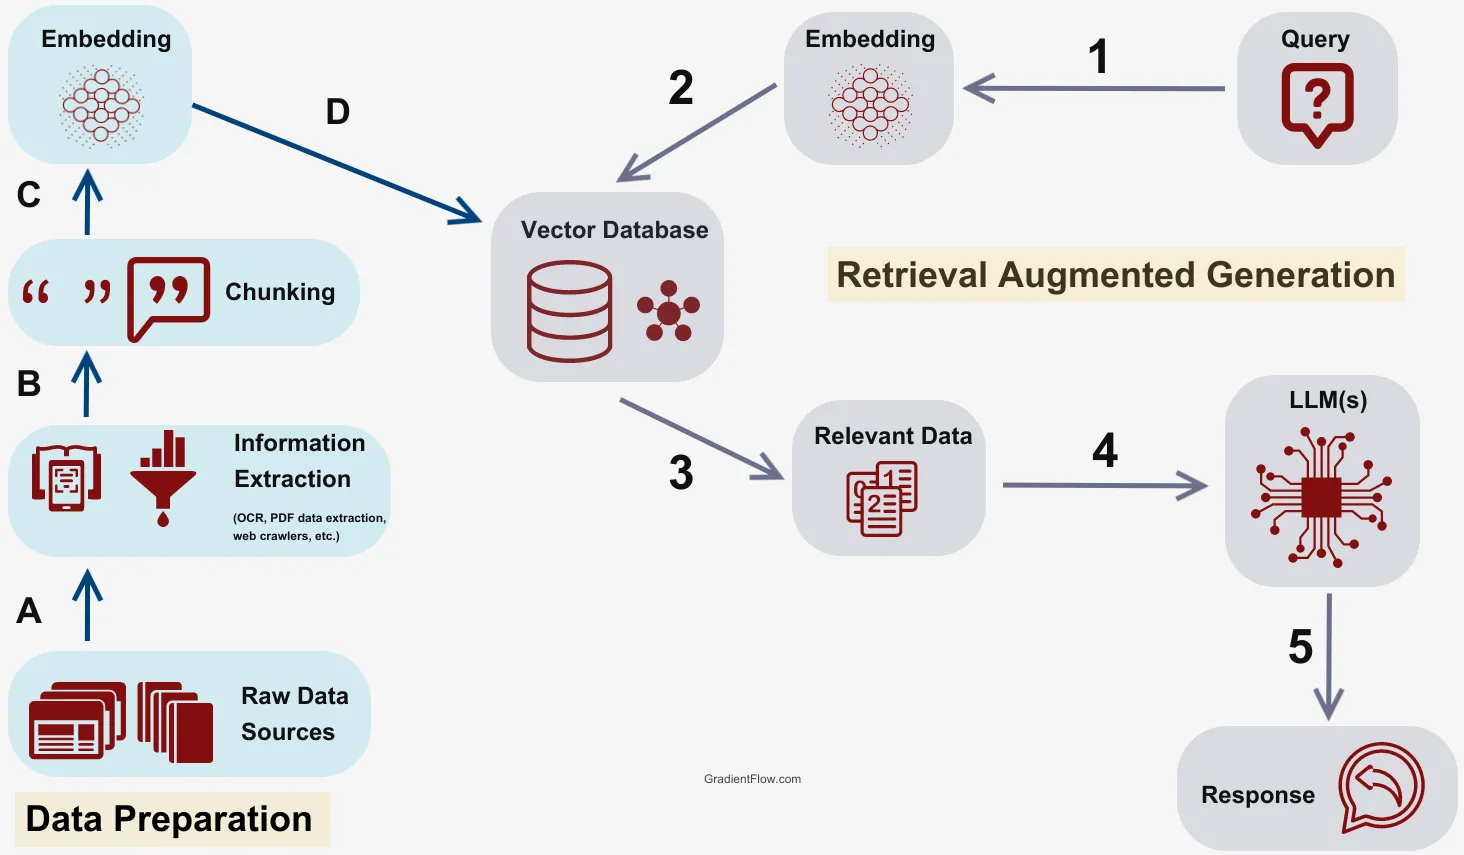
\includegraphics[width=\textwidth]{RAG.png}
		\centering
	\end{figure}
\end{displayquote}
\newpage

RAG kan hier dienst doen als een mogelijke plaatsvervanger voor manuele research en het opstellen van communicatiedocumenten (zoals aangetekende brieven, invorderingen, ...). Deze optie zal in
een later stadium van deze bachelorproef geëvealueerd worden. Advocatuur is een heel toepasselijk gebied voor RAG:

\begin{displayquote}
	Practically, RAG is likely preferable in environments like
	legal, customer service, and financial services where the ability to
	dynamically pull vast amounts of up-to-date data enables the most accurate and comprehensive responses.
\end{displayquote}



%%=============================================================================
%% Methodologie
%%=============================================================================

\chapter{\IfLanguageName{dutch}{Methodologie}{Methodology}}%
\label{ch:methodologie}

%% TODO: In dit hoofstuk geef je een korte toelichting over hoe je te werk bent
%% gegaan. Verdeel je onderzoek in grote fasen, en licht in elke fase toe wat
%% de doelstelling was, welke deliverables daar uit gekomen zijn, en welke
%% onderzoeksmethoden je daarbij toegepast hebt. Verantwoord waarom je
%% op deze manier te werk gegaan bent.
%% 
%% Voorbeelden van zulke fasen zijn: literatuurstudie, opstellen van een
%% requirements-analyse, opstellen long-list (bij vergelijkende studie),
%% selectie van geschikte tools (bij vergelijkende studie, "short-list"),
%% opzetten testopstelling/PoC, uitvoeren testen en verzamelen
%% van resultaten, analyse van resultaten, ...
%%
%% !!!!! LET OP !!!!!
%%
%% Het is uitdrukkelijk NIET de bedoeling dat je het grootste deel van de corpus
%% van je bachelorproef in dit hoofstuk verwerkt! Dit hoofdstuk is eerder een
%% kort overzicht van je plan van aanpak.
%%
%% Maak voor elke fase (behalve het literatuuronderzoek) een NIEUW HOOFDSTUK aan
%% en geef het een gepaste titel.

In dit hoofdstuk volgt wat er precies zal gebeuren om een RAG client app te bouwen die toepasbaar kan zijn voor grote datasets zoals die van Deltalex Advocaten. 
De volgende hoofdstukken zullen uitgebreid beschreven, onderzocht en uitgetest worden. \\

Het onderzoek naar oplossingen is parallel gevoerd samen met het opbouwen van een stappenplan om een werkende generieke digitale assistent te bekomen. 
Eerst worden de stappen van het onderzoek overlopen, dan gaan we naadloos over naar onderzoek over welke stappen en technologieën er aan bod komen in de ontwikkeling van een digitale assistent. 

\begin{enumerate}
    \item \textbf{Onderzoek: Requirements-analyse}
    \item \textbf{Onderzoek: Literatuurstudie}
    \item \textbf{Onderzoek: Haalbaarheid en dataveiligheid} 

    \item \textbf{Development: Documentdatabase}
    \item \textbf{Development: Context-aware chunking van verzamelde data}
    \item \textbf{Development: Integreren van Ollama met documentdatabase}
    \item \textbf{Development: Implementeren van een chatfrontend}
    \item \textbf{Development: Opzetten van lokale omgeving en componenten verbinden}
    \item \textbf{Development: Optimaliseren en testen}  

    \item \textbf{Resultaten}
\end{enumerate} 

%%Op het einde van deze reis is de uitkomst een digitale assistent die kennis heeft van alle dossierdata van een hypothetisch advocatenkantoor. 
%%Deze zal advocaten helpen met het opzoeken van informatie, opstellen van brieven, communicatie en dergelijke. 




% Voeg hier je eigen hoofdstukken toe die de ``corpus'' van je bachelorproef
% vormen. De structuur en titels hangen af van je eigen onderzoek. Je kan bv.
% elke fase in je onderzoek in een apart hoofdstuk bespreken.

%\input{...}
%\input{...}
%...

%%=============================================================================
%% Conclusie
%%=============================================================================

\chapter{Conclusie}%
\label{ch:conclusie}

% TODO: Trek een duidelijke conclusie, in de vorm van een antwoord op de
% onderzoeksvra(a)g(en). Wat was jouw bijdrage aan het onderzoeksdomein en
% hoe biedt dit meerwaarde aan het vakgebied/doelgroep? 
% Reflecteer kritisch over het resultaat. In Engelse teksten wordt deze sectie
% ``Discussion'' genoemd. Had je deze uitkomst verwacht? Zijn er zaken die nog
% niet duidelijk zijn?
% Heeft het onderzoek geleid tot nieuwe vragen die uitnodigen tot verder 
%onderzoek?

De uitkomst van dit onderzoek is een roadmap die informatie bevat over iedere component van de opbouw van een digitale assistent. 
Eerst was de opzet van dit onderzoek om een assistent te implementeren en te integreren met bestaande software. 

Natuurlijk werkt deze assistent met libraries en componenten die toch heel wat resources gebruiken om vloeiend te bouwen, draaien en testen. 
Dit in combinatie met de gevoeligheid van de cliëntdata is de beslissing gekomen om dit onderzoek puur hypothetisch uit te voeren. 
Denk over dit onderzoek als een stappenplan om een lezer bekend te maken met de basisconcepten van Natural Language Processing, Large Language Models, Retrieval Augmented Generation en meer. 

Veel stappen uit dit onderzoek worden minder breed besproken gezien het hedendaagse aanbod van digitale tools zoals JavaScript libraries, 
frameworks die al heel goeie implementaties voor digitale assistenten leveren en de extraordinaire snelle aard van verandering van het huidig technologisch spectrum. 

Er is in dit onderzoek geprobeerd om zo veel mogelijk technologiespecifiek te werken. 
Het kan goed zijn dat er binnenkort betere technologieën uitgebracht worden die veel beter presteren dan degene die hier gebruikt worden. 
De technologieën gebruikt in dit onderzoek zijn op het moment van onderzoek de meest geschikte en performante op de markt, waarvan de meeste open-source. 

In conclusie hoop ik dat een lezer van dit onderzoek enerzijds bijleert over digitale assistenten en hoe ze werken onder de motorkap. 
Anderzijds dat hij het ook kan gebruiken als stappenplan tijdens het implementeren van zijn eigen assistent, iets waar de student die er nu aan werkt ook zeker gebruik van zal maken. 


%---------- Bijlagen -----------------------------------------------------------

\appendix

\chapter{Onderzoeksvoorstel}

Het onderwerp van deze bachelorproef is gebaseerd op een onderzoeksvoorstel dat vooraf werd beoordeeld door de promotor. Dat voorstel is opgenomen in deze bijlage.

%% TODO: 
%\section*{Samenvatting}

% Kopieer en plak hier de samenvatting (abstract) van je onderzoeksvoorstel.

% Verwijzing naar het bestand met de inhoud van het onderzoeksvoorstel
%---------- Inleiding ---------------------------------------------------------
\section{Introductie}%
\label{sec:introductie}

Mijn bachelorproef spitst zich toe op het optimaliseren van de administratieve workload bij advocatenkantoor Deltalex. Dit zal gebeuren via het invoeren van geautomatiseerde processen, het
ontwikkelen van een centrale webinterface om opzoekwerk te verrichten, daarbij ook een portaal om de sjablonen van de meestgebruikte documenten bij te houden en te bewerken.

Dit onderzoek vindt zijn oorsprong in de vaststelling van veel tijdrovende en repetitieve taken die de efficiëntie van dit kantoor kunnen belemmeren,
zoals het handmatig opzoeken van cliëntgegevens in openbare databases en het bijwerken van veelgebruikte documenttemplates.

De onderzoeksvraag van mijn bachelorproef luidt: "Hoe kunnen geautomatiseerde processen, in combinatie met een webinterface voor beheer, de administratieve
last in advocatenkantoren verminderen en de efficiëntie bevorderen?"

Het beoogde eindresultaat omvat niet alleen een werkend prototype van automatisatie en de bijbehorende webinterface,
maar ook een grondig rapport met aanbevelingen voor implementatie in advocatenkantoren.

Het succes van deze bachelorproef zal worden beoordeeld aan de hand van daadwerkelijke verbeteringen in efficiëntie en
tijdsbesparing binnen advocatenkantoor Deltalex.

%---------- Stand van zaken ---------------------------------------------------
\section{Literatuurstudie: automatisatie en de selectie van CMS's in de advocatuur}%
\label{sec:state-of-the-art}

Consider one real-world example: if your firm had 12,000 documents to review, and each one had 75 questions to answer, the task will take weeks to complete. Even with a sizable team working in concert, the sheer volume of work is daunting. One of those, “Where do I even start?” types of tasks others might shrink from.
But what if you started by working the process, not just digging into the work? By automating even a part of a task that large, you stand to shave hours off the time involved.
\autocite{ThomsonReuters2023}

Deze citatie illustreert dat investeren in een efficiëntere aanpak van je repetitieve taken zeker kan lonen. Dit is natuurlijk ook toepasbaar op een advocatenkantoor, volgende citatie illustreert het maken van documenten, waaronder dagvaardingen, invorderingen en mails.

Document creation, for example, requires a large amount of repetitive work. Diving right into the work may seem like the best way to get ahead, but by taking the time to define the fields in a document, and set up corresponding variables, it’s easy for a computer to automatically create custom, accurate documents on a scale that no human can match.
\autocite{ThomsonReuters2023}

Automatisatie kan ook executie van taken zoals indienprocedures en legal research exponentieel sneller maken. \autocite{Aston2023}

Het huidige landschap van administratieve\\ tools is heel groot. In het geval van Deltalex (en andere kantoren) hebben ze gekozen voor een bepaald softwarepakket. Dit is veelal een moeilijke keuze omdat er heel veel pakketten beschikbaar zijn en deze bieden elk hun voor- en nadelen. De selectie van een dergelijke tool kan een moeizaam proces zijn, maar kan gegoten worden in volgende stappen.
\autocite{Clio2023}

\begin{itemize}
	\item \emph{Kies tussen cloud- of lokale opslag:} Waar hosten? 
        \item \emph{Bekijk de kosten- en onderhoudsverschillen:} Varieert sterk op basis van stap 1.
        \item \emph{Zorg voor toegang tot informatie op afstand:} Veel advocaten werken soms op afstand, bv. vanuit een rechtbank.
        \item \emph{Controleer de compatibiliteit met bestaande software:}\\ Complexere pakketten worden meestal pas aangekocht als het kantoor zich verder bevindt dan de startfase. M.a.w. er is zeker al bestaande data op oudere systemen.
        \item \emph{Evalueer gebruiksgemak en trainingsvereisten:} Het is belangrijk dat iedere gebruiker zo snel en probleemloos met de nieuwe software aan de slag kan.
        \item \emph{Zorg voor ethische naleving en beveiliging:} Advocatenkantoren werken onder strikte regels voor professioneel gedrag, daarom is het aangeraden om voor gespecialiseerde software te opteren.
\end{itemize}

Dergelijke pocessen kunnen lang duren en in het geval van Deltalex is dit al gebeurd. Daarom bespreek ik in deze bachelorproef de ontwikkeling van een externe interface om specifieke taken sneller af te handelen.

%---------- Methodologie ------------------------------------------------------
\section{Methodologie}%
\label{sec:methodologie}
Deze bachelorproef zal een combinatie zijn van een case study in advocatenkantoor Deltalex en een proof of concept van het platform om in het kantoor de administratieve workload zoveel mogelijk te minimaliseren. Deze implementatie valideert de haalbaarheid en de effectiviteit van de oplossing doorheen heel het kantoor, beginnende bij één specifieke advocaat. 

Het onderzoek zal zich concentreren op accurate en objectieve resultaten en vermijdt onderzoekstechnieken die subjectieve data yielden, zoals enquêtes. Literatuurstudie, interviews en praktische data zullen de bouwstenen zijn van het uiteindelijke verdict van de implementatie. 

De voorgaande technische analyse zal voor mij een unieke kans zijn om op zowel het informaticadomein als in de administratieve/ juridische sector mijn skills bij te scherpen. Er zullen tools gebruikt worden als front-end-webassembly talen voor een moderne approach van een webinterface. Voor automatisatie van queries online zal er gebruik gemaakt worden van scripttalen en er zal ook grondig uitgezocht worden hoe men sjablonen zo effectief mogelijk kan aanpassen via MS Office XML-injecties in documenten. 

Deze proef zal 12 weken in beslag nemen en is optimaal zoals onderstaand ingedeeld:
\begin{itemize}
        \item Requirementanalyse: 2 weken.\\ \emph{Deliverable} -> Verslag van requirements
        \item Ontwerp en technologieselectie: 2 weken.\\ \emph{Deliverable} -> technologiestack en praktische planning voor implementatie
        \item Implementatie: 4 weken.\\ \emph{Deliverable} -> werkende proof of concept
        \item Evaluatie: 2 weken. \\ \emph{Deliverable} -> Evaluatierapport
        \item Aanpassen van project en conclusie: 2 weken.\\ \emph{Deliverable} -> Aangepaste proof of concept, eindrapport en conclusie
\end{itemize}

%---------- Verwachte resultaten ----------------------------------------------
\section{Verwacht resultaat, conclusie}%
\label{sec:verwachte_resultaten}
Ik verwacht natuurlijk dat Deltalex geniet van mijn oplossing en dat alle vennoten hun tijd kunnen investeren in dingen die écht belangrijk zijn. Daarmee vermijden ze repetitieve taken die heel tijdrovend zijn. Ook zal de stress en frustratie op de werkvloer afnemen. Dat zal resulteren in een aangename werkomgeving waar iedereen zich productief bezighoudt en zichzelf amuseert in hun werk.

Naar de praktische kant toe verwacht ik drie dingen:
\begin{itemize}
        \item \emph{Requirementsanalyse}
        \item \emph{Ontwerp en implementatie van gekozen technologieën}
        \item \emph{Evaluatie en validatie}
\end{itemize}

Ik hoop ook dat mijn bachelorproef kan motiveren waarom een kantoor (in dit geval advocatenkantoor) voordeel zou kunnen halen uit specifieke implementaties, die kunnen helpen aan bepaalde nicheproblemen, zonder een volledig nieuw systeem te implementeren. Een nieuw systeem moet aangekocht, aangeleerd en aangepast worden. Dit is een kwestie van hoge kosten, potentieel lange gewenning en mogelijke datamigratieproblemen. 


%%---------- Andere bijlagen --------------------------------------------------
% TODO: Voeg hier eventuele andere bijlagen toe. Bv. als je deze BP voor de
% tweede keer indient, een overzicht van de verbeteringen t.o.v. het origineel.
%\input{...}

%%---------- Backmatter, referentielijst ---------------------------------------

\backmatter{}

\setlength\bibitemsep{2pt} %% Add Some space between the bibliograpy entries
\printbibliography[heading=bibintoc]

\end{document}
